%%%%%%%%%%%%%%%%%%%%%%%%%%%%%%%%%%%%%%%%%%%
%%%%%%%%%%%%%%%%%%%%%%%%%%%%%%%%%%%%%%%%%%%
%%%%%%%%%%%%%%% CHAPTER 01 %%%%%%%%%%%%%%%%


\section{Introdução à Modelagem de Sistemas Dinâmicos}

\frame{
\frametitle{Objetivo do curso}
\begin{block}{}
O principal objetivo deste curso é apresentar os \textbf{fundamentos matemáticos para controle} de sistemas lineares, apresentando as principais ferramentas de \textbf{modelagem}, bem como utilizando \textbf{leis físicas} pertinentes a cada problema físico em estudo.
\end{block}
}

\frame{
\frametitle{Definições}
\begin{block}{Sistema}
\begin{itemize}
    \item Um \textbf{sistema} é qualquer conjunto de componentes que \textbf{interagem entre si} para o qual existe uma relação de causa e efeito entre as variáveis.
    \item É importante perceber que devemos considerar a \textbf{interação das variáveis} na modelagem de um sistema, e não apenas tratar os elementos de forma separada.
    \begin{itemize}
        \item \textbf{Exemplo}: no \textit{design} de um circuito eletrônico, temos que considerar a parte mecânica (sistema mecânico), mas também a dissipação de calor gerado (sistema térmico).
    \end{itemize}
\end{itemize}
\end{block}
}

\frame{
\frametitle{Definições}
\begin{block}{Sistema dinâmico}
\begin{itemize}
    \item Um sistema é dito \textbf{estático} quando a saída atual do sistema só depende da entrada atual, isto é, a saída do sistema só varia se a entrada do sistema variar (não é dependente do tempo).
    \begin{itemize}
        \item \textbf{Exemplo}: divisor de tensão alimentado por uma fonte de tensão constante.
    \end{itemize}
    \item Um sistema é dito \textbf{dinâmico} se sua saída depende da entrada e dos valores passados da entrada. Num sistema dinâmico a saída varia se ela não estiver num ponto de equilíbrio, mesmo que nenhuma entrada esteja sendo aplicada (é dependente do tempo).
    \begin{itemize}
        \item \textbf{Exemplo}: valor, em reais, em uma conta corrente.
    \end{itemize}
\end{itemize}
\end{block}
}

\frame{
\frametitle{Definições}
\begin{block}{Modelagem}
\begin{itemize}
    \item Um \textbf{modelo matemático} é a descrição de um sistema em termos de \textbf{equações}. É um dispositivo que de alguma maneira descreve o \textbf{comportamento do sistema}.
    \item Deste modo, modelar significa representar o Sistema Físico Real (SFR), ou parte dele, em forma física ou simbólica, para predizer ou descrever o seu comportamento. 
    \item Portanto, \textbf{modelagem} é o ato de modelar, ou seja, é a atividade de construir o modelo para representar o SFR.
\end{itemize}
\end{block}
}

\frame{
\frametitle{Modelos Matemáticos}
\centerline{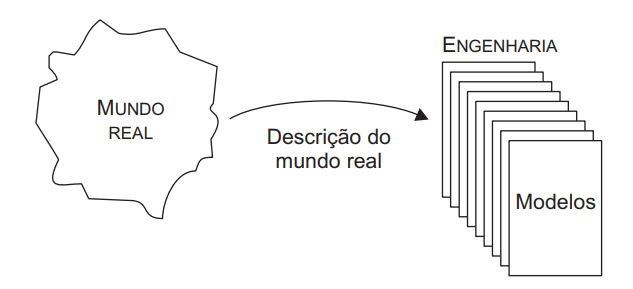
\includegraphics[width=0.9\linewidth]{Figuras/Ch01/fig5.PNG}}
}

\frame{
\frametitle{Modelos Matemáticos}
\begin{block}{Caixa branca}
\begin{itemize}
    \item Também conhecido como \textbf{modelagem física}, o processo de obtenção do modelo se baseia em \textbf{leis e princípios físicos}.
    \item Neste tipo de modelo, apenas as variáveis de \textbf{entrada} e a \textbf{física} do sistema são considerados.
    \item Além disso, todos os parâmetros são conhecidos, ou previamente determinados.
    \item Os dados de entrada e saída do sistema, quando disponíveis, são usados apenas para \textbf{validar} o modelo.
\end{itemize}
\end{block}
}

\frame{
\frametitle{Modelos Matemáticos}
\begin{block}{Caixa preta}
\begin{itemize}
    \item Também conhecido como \textbf{modelagem por identificação de sistemas}, o processo de obtenção do modelo se baseia em \textbf{dados experimentais coletados}.
    \item Neste tipo de modelo, apenas as variáveis de \textbf{entrada} e a \textbf{saída} do sistema são considerados.
    \item Nenhuma informação sobre o sistema está disponível além dos \textbf{dados} ou, se disponível, não é usada no procedimento de obtenção do modelo. 
\end{itemize}
\end{block}
}

\frame{
\frametitle{Modelos Matemáticos}
\begin{block}{Caixa cinza}
\begin{itemize}
    \item Modelagem que considera tanto as variáveis de \textbf{entrada} e a \textbf{saída} do sistema, como alguma \textbf{informação auxiliar} do sistema.
    \item Esta informação auxiliar pode ser desde a função de ativação, no caso de redes neurais, até leis físicas e parâmetros estimados.
    \item Os modelos caixa cinza, à semelhança dos caixa preta, têm \textbf{menos significado físico} que os caixa branca. Note que, se a informação auxiliar disponível for incorreta, seu uso na identificação caixa cinza será conflituoso com os dados, podendo resultar em um modelo de baixa qualidade. Tal fato não ocorre na identificação caixa preta.
\end{itemize}
\end{block}
}

\frame{
\frametitle{Modelos Matemáticos}
\centerline{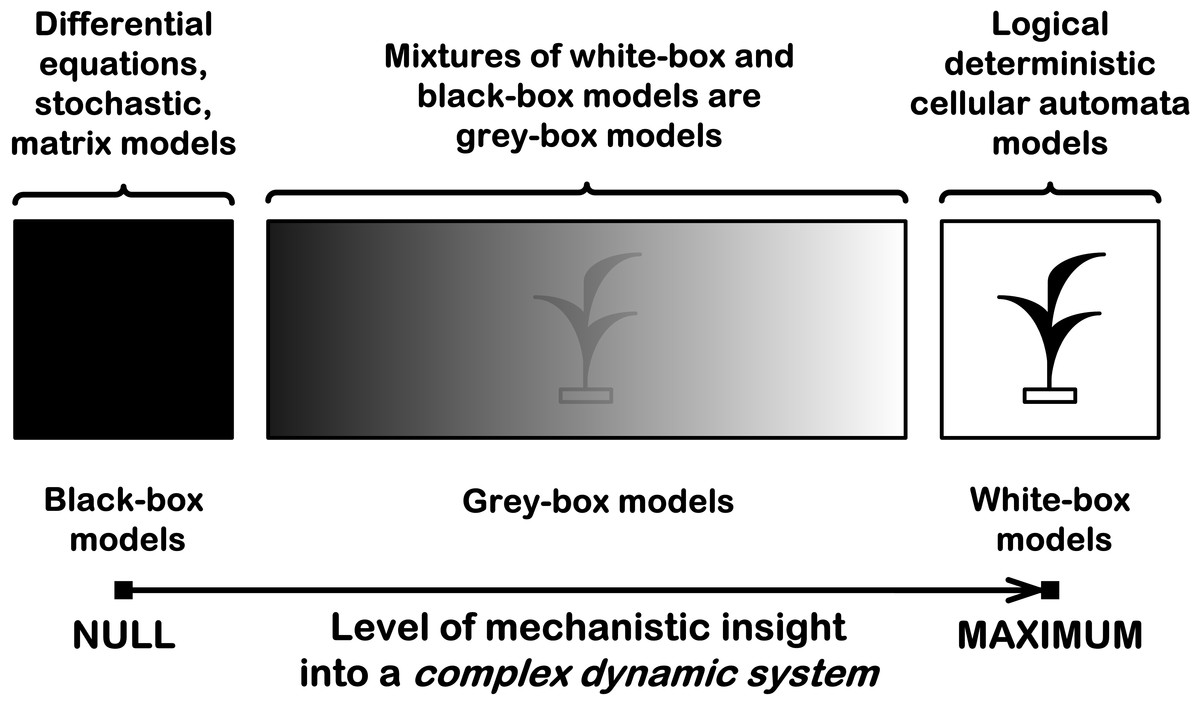
\includegraphics[width=0.9\linewidth]{Figuras/Ch01/fig6.jpg}}
}

\frame{
\frametitle{Visão geral da modelagem}
\centerline{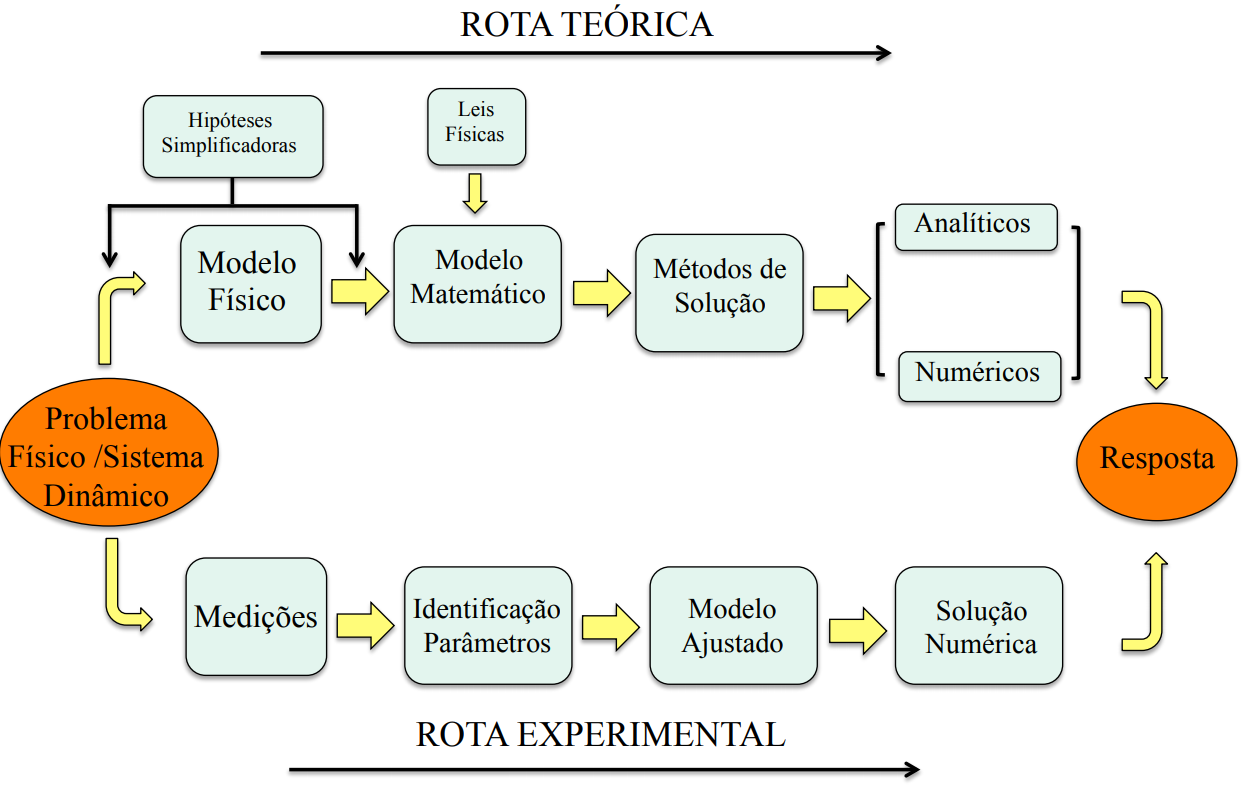
\includegraphics[width=1\linewidth]{Figuras/Ch01/fig1.PNG}}
}

\frame{
\frametitle{Validação do modelo}
\begin{block}{Definição}
\begin{itemize}
    \item A \textbf{validação} de um modelo matemático (que representa um SFR) consiste em checar se este comporta-se como o mundo real sob as mesmas condições. Em outras palavras, \textbf{o modelo obtido serve? Ele é suficientemente bom?}
    \end{itemize}
\end{block}
}

\frame{
\frametitle{Simulação do modelo}
\begin{block}{Definição}
\begin{itemize}
    \item Comparar a \textbf{simulação} do modelo obtido com dados medidos é provavelmente a forma mais usual de se validar um modelo.
    \item Durante o processo de validação \textbf{não se devem usar os dados utilizados para obter o modelo}.
    \end{itemize}
\end{block}
}

\frame{
\frametitle{Solução do modelo}
\begin{block}{Abstração matemática}
\begin{itemize}
    \item Não se pode esquecer que o modelo que está sendo analisado é uma descrição matemática \textbf{aproximada} do sistema, e não o sistema físico em si.
    \item Conclusões baseadas em equações que precisam de uma gama de \textbf{hipóteses e simplificações} pode ou não ser aplicada no sistema atual.
\end{itemize}
\end{block}
}

\frame{
\frametitle{Fluxograma}
\centerline{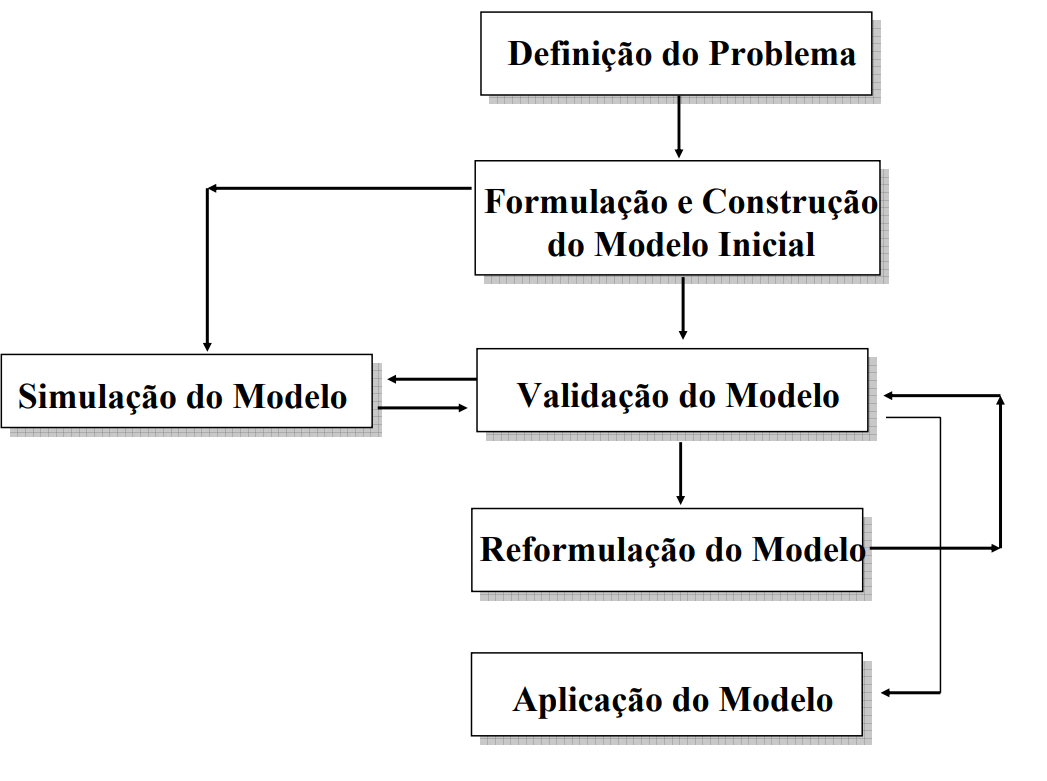
\includegraphics[width=0.8\linewidth]{Figuras/Ch01/fig7.PNG}}
}

\frame{
\frametitle{O conceito de entrada e saída}
\centerline{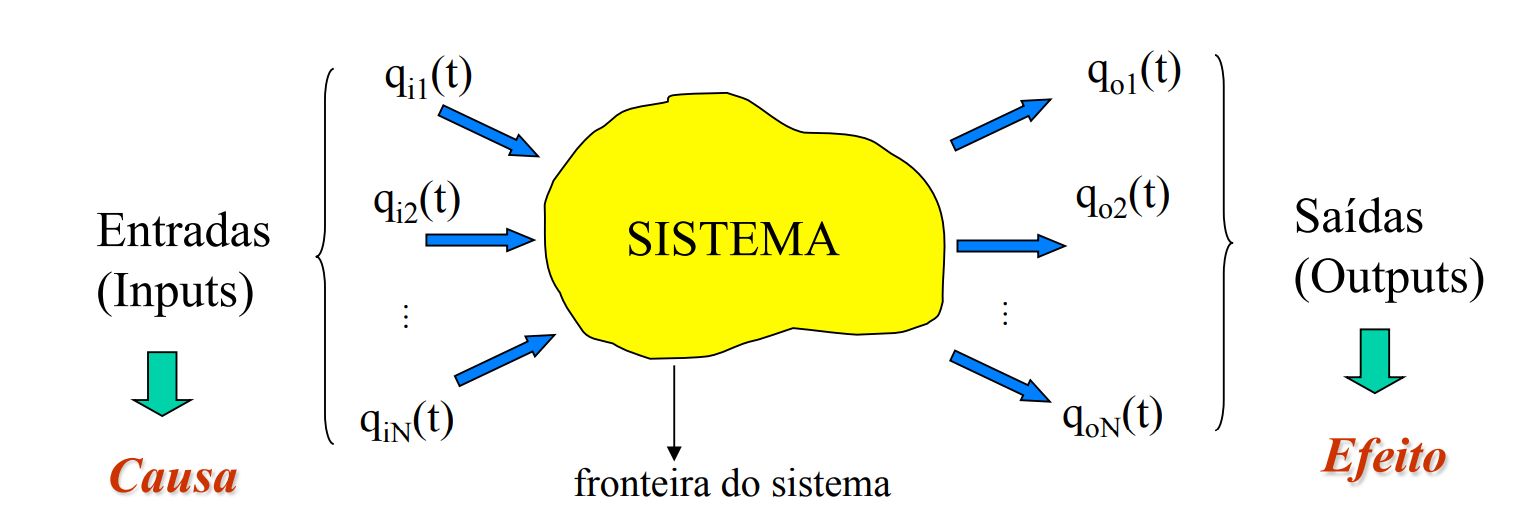
\includegraphics[width=1\linewidth]{Figuras/Ch01/fig2.PNG}}
\begin{block}{}
\begin{itemize}
    \item O sistema geralmente é representado por uma caixa (\textbf{caixa preta}).
    \item \textbf{Entradas}: são agentes que provocam distúrbio no sistema. 
    \begin{itemize}
        \item \textbf{Exemplo}: força aplicada a uma massa.
    \end{itemize}
    \item \textbf{Saídas}: são variáveis que são calculadas ou medidas.
    \begin{itemize}
        \item \textbf{Exemplo}: velocidade de uma massa.
    \end{itemize}
\end{itemize}
\end{block}
}

\frame{
\frametitle{Classificação de sistemas}
\begin{block}{Sistemas com parâmetros concentrados ou distribuídos}
\begin{itemize}
    \item Em um sistema com \textbf{parâmetros distribuídos}, a excitação e a resposta dependem do tempo e das coordenadas espaciais, logo são descritos por \textbf{equações diferenciais parciais} (mais de uma variável independente).
    \begin{itemize}
        \item \textbf{Exemplo}: ângulo depende do torque aplicado e da distância até a parede.
    \end{itemize}
    \item Em um sistema com \textbf{parâmetros concentrados}, a excitação e a resposta dependem apenas do tempo, logo são descritos por \textbf{equações diferenciais ordinárias}.
    \begin{itemize}
        \item \textbf{Exemplo}: ângulo depende apenas do torque aplicado - momento de inércia $J$ representa a massa distribuída.
    \end{itemize}
\end{itemize}
\end{block}
\centerline{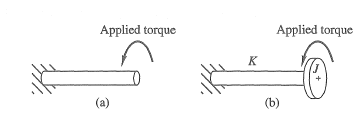
\includegraphics[width=0.6\linewidth]{Figuras/Ch01/fig3.PNG}}
}

\frame{
\frametitle{Classificação de sistemas}
\begin{block}{Sistemas contínuos ou discretos}
\begin{itemize}
    \item Um sistema \textbf{contínuo no tempo} é aquele cujas entradas e saídas são definidas sobre um intervalo de tempo contínuo. Tais sistemas são descritos por \textbf{equações diferenciais}.
    \item Já um sistema \textbf{discreto no tempo} possui variáveis que são determinadas em diferentes instantes de tempo (o que acontece entre estes instantes não é definido ou não é de interesse). Tais sistemas são descritos por \textbf{equações de diferenças}.
\end{itemize}
\end{block}
\centerline{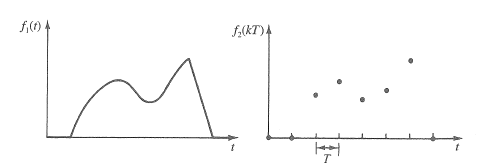
\includegraphics[width=0.7\linewidth]{Figuras/Ch01/fig4.PNG}}
}

\frame{
\frametitle{Classificação de sistemas}
\begin{block}{Sistemas variantes no tempo ou invariantes no tempo}
\begin{itemize}
    \item No modelo matemático, i.e., nas equações diferenciais, os parâmetros do sistema aparecem sob forma de coeficientes. Se os coeficientes são constantes, dizemos que o sistema \textbf{é invariante no tempo}.
    \begin{itemize}
        \item \textbf{Exemplo}: Pêndulo.
    \end{itemize}
    \item Caso contrário, o sistema é considerado \textbf{variante no tempo}.
    \begin{itemize}
        \item \textbf{Exemplo}: foguete na
    sua fase propulsada, pois o mesmo perde massa durante a queima de combustível. 
    \end{itemize}
\end{itemize}
\end{block}
}

\frame{
\frametitle{Classificação de sistemas}
\begin{block}{Sistemas lineares ou não lineares}
\begin{itemize}
    \item Um sistema linear é aquele que obedece a \textbf{propriedade da superposição}:
    \begin{enumerate}
        \item Multiplicar as entradas por qualquer constante $\alpha$ implica em multiplicar as saídas por $\alpha$ (\textbf{princípio da homogeneidade}).
        \item A resposta a várias entradas aplicadas simultaneamente deve ser a soma das respostas individuais a cada entrada aplicada separadamente (\textbf{princípio da aditividade}).
    \end{enumerate}
    $$a_1 \diff{y}{t} + a_0 y(t) = b_0 u(t)$$
    %\diff*[4]{g}{t}{t = 1}
    \item Caso contrário, o sistema é considerado \textbf{não linear}.
    \begin{itemize}
        \item Restrições podem ser aplicadas? \textbf{Linearização}.
    \end{itemize}
    $$\diff{y}{t} + u(t)y(t) = u(t)$$
\end{itemize}
\end{block}
}

\frame{
\frametitle{Exercícios}
\begin{block}{}
01. Uma companhia de automóveis contratou uma empresa de engenharia para análise do funcionamento do sistema de suspensão de um dos seus veículos, conforme mostra a figura. Você, na função de Engenheiro de Controle e Automação, deve avaliar se o sistema pneu/suspensão de um carro está funcionando corretamente, sem gastar muito dinheiro e sem colocar em risco a vida das pessoas. Como você faria isso? Descreva todas as etapas.
\end{block}
\centerline{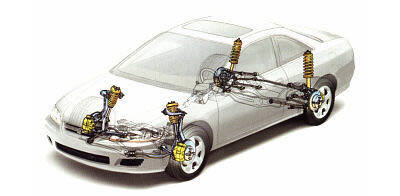
\includegraphics[width=0.7\linewidth]{Figuras/Ch01/fig8.jpg}}
}

\frame{
\frametitle{Exercícios}
\begin{block}{}
02. Para entender e controlar sistemas complexos, devemos obter modelos matemáticos quantitativos destes sistemas. É portanto necessário analisar as relações entre as variáveis do sistema. Descreva, em forma de tópicos, a abordagem mais usual para a análise de um sistema qualquer, isto é, quais são os passos necessários para projetar um sistema de controle.
\end{block}
}

\frame{
\frametitle{Referências e exercícios complementares}
\begin{itemize}
\item CLOSE, Charles M.; FREDERICK, Dean K.; NEWELL, Jonathan C. Modeling and Analysis of Dynamic Systems, 3 ed. John Wiley \& Sons, 2003.
\end{itemize}
\centering{\alert{Página 1 - \textbf{Capítulo 1}}} \\
}